\subsection{Test HTTP Methods - OTG-CONFIG-006}

\subsubsection{BANK-APP}
\begin{longtable}[l]{ p{2.3cm} | p{.79\linewidth} }\hline
    & \textbf{BANK-APP} \\ \hline
    \textbf{Observation} & It was observed that the server allows only 4 methods : HEAD, GET, POST, OPTIONS. \\
    \textbf{Discovery} & We used the Nmap tool to identify the HTTP methods that are allowed by the server. See Figure \ref{fig:nmap_http_methods}. We found that there is no TRACE method allowed by the server. So there is no chance of Cross Site Tracing(XST) attacks. Methods like HEAD were explored with Advance Rest Client Tool to bypass authentication but without success. \\
    \textbf{Likelihood} & N/A \\
    \textbf{Impact} & N/A \\
    \textbf{Recommen\-dations} & N/A \\ \hline
    \textbf{CVSS} & N/A
    \\ \hline
\end{longtable}

\subsubsection{SecureBank}
\begin{longtable}[l]{ p{2.3cm} | p{.79\linewidth} }\hline
    & \textbf{SecureBank} \\ \hline
    \textbf{Observation} & It was observed that the server allows only 4 methods : HEAD, GET, POST, OPTIONS. \\
    \textbf{Discovery} & Same as described for BANK-APP. \\
    \textbf{Likelihood} & N/A \\
    \textbf{Impact} & N/A \\
    \textbf{Recommen\-dations} & recommendations \\ \hline
    \textbf{CVSS} & N/A
    \\ \hline
\end{longtable}

\subsubsection{Comparison}
Both applications exhibit similar behavior with respect to the allowed HTTP methods and neither contain any vulnerabilty.
\\
\begin{figure}[ht]
	\centering
		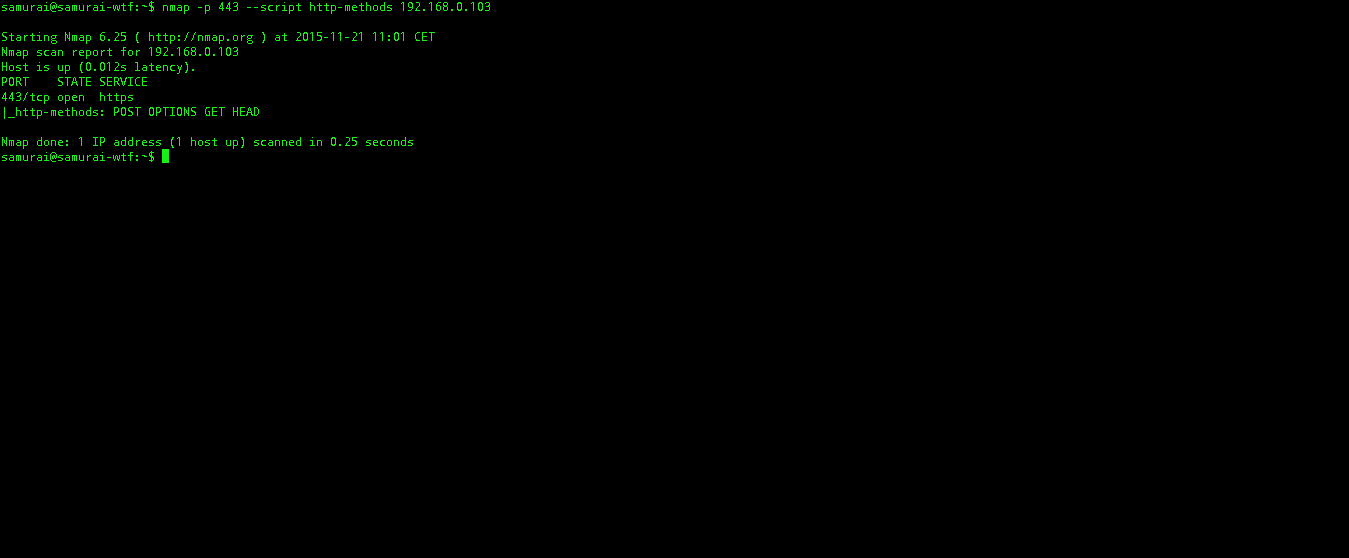
\includegraphics[width=.8\linewidth]{figures/OTG-CONFIG-006.png}
		\caption{Nmap - Check for allowed HTTP methods}
	\label{fig:nmap_http_methods}
\end{figure}

\clearpage